% Options for packages loaded elsewhere
\PassOptionsToPackage{unicode}{hyperref}
\PassOptionsToPackage{hyphens}{url}
%
\documentclass[
  9pt,
  landscape]{article}
\usepackage{amsmath,amssymb}
\usepackage{lmodern}
\usepackage{iftex}
\ifPDFTeX
  \usepackage[T1]{fontenc}
  \usepackage[utf8]{inputenc}
  \usepackage{textcomp} % provide euro and other symbols
\else % if luatex or xetex
  \usepackage{unicode-math}
  \defaultfontfeatures{Scale=MatchLowercase}
  \defaultfontfeatures[\rmfamily]{Ligatures=TeX,Scale=1}
\fi
% Use upquote if available, for straight quotes in verbatim environments
\IfFileExists{upquote.sty}{\usepackage{upquote}}{}
\IfFileExists{microtype.sty}{% use microtype if available
  \usepackage[]{microtype}
  \UseMicrotypeSet[protrusion]{basicmath} % disable protrusion for tt fonts
}{}
\makeatletter
\@ifundefined{KOMAClassName}{% if non-KOMA class
  \IfFileExists{parskip.sty}{%
    \usepackage{parskip}
  }{% else
    \setlength{\parindent}{0pt}
    \setlength{\parskip}{6pt plus 2pt minus 1pt}}
}{% if KOMA class
  \KOMAoptions{parskip=half}}
\makeatother
\usepackage{xcolor}
\usepackage[margin=2cm]{geometry}
\usepackage{graphicx}
\makeatletter
\def\maxwidth{\ifdim\Gin@nat@width>\linewidth\linewidth\else\Gin@nat@width\fi}
\def\maxheight{\ifdim\Gin@nat@height>\textheight\textheight\else\Gin@nat@height\fi}
\makeatother
% Scale images if necessary, so that they will not overflow the page
% margins by default, and it is still possible to overwrite the defaults
% using explicit options in \includegraphics[width, height, ...]{}
\setkeys{Gin}{width=\maxwidth,height=\maxheight,keepaspectratio}
% Set default figure placement to htbp
\makeatletter
\def\fps@figure{htbp}
\makeatother
\setlength{\emergencystretch}{3em} % prevent overfull lines
\providecommand{\tightlist}{%
  \setlength{\itemsep}{0pt}\setlength{\parskip}{0pt}}
\setcounter{secnumdepth}{-\maxdimen} % remove section numbering
\ifLuaTeX
  \usepackage{selnolig}  % disable illegal ligatures
\fi
\IfFileExists{bookmark.sty}{\usepackage{bookmark}}{\usepackage{hyperref}}
\IfFileExists{xurl.sty}{\usepackage{xurl}}{} % add URL line breaks if available
\urlstyle{same} % disable monospaced font for URLs
\hypersetup{
  hidelinks,
  pdfcreator={LaTeX via pandoc}}

\author{}
\date{\vspace{-2.5em}}

\begin{document}

\hypertarget{time-instant-318-capacity500-leafs247-epsilon4.}{%
\subsection{Time instant : 318 (capacity=500, leafs=247,
epsilon=4).}\label{time-instant-318-capacity500-leafs247-epsilon4.}}

\begin{minipage}{0.5\textwidth} 
\centering 
\begin{tabular}{rrrrrrr}
  \hline
 & Min. & 1st Qu. & Median & Mean & 3rd Qu. & Max. \\ 
  \hline
stats & 4.00 & 117.50 & 179.00 & 206.37 & 271.50 & 519.00 \\ 
   \hline
\end{tabular}
\vspace{0.5cm} 


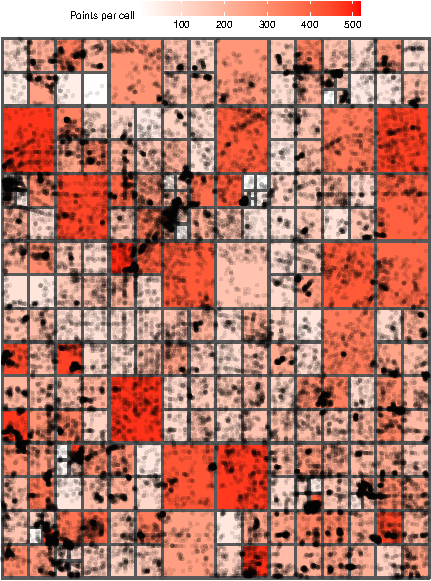
\includegraphics[width=1\linewidth,height=0.8\textheight]{distance_files/figure-latex/p1_318_500_4-1} 

\end{minipage} 
\begin{minipage}{0.5\textwidth} 
\centering 
\begin{tabular}{rrrrrrr}
  \hline
 & Min. & 1st Qu. & Median & Mean & 3rd Qu. & Max. \\ 
  \hline
stats & 0.00 & 2.50 & 9.00 & 41.08 & 19.00 & 1649.00 \\ 
   \hline
\end{tabular}
\vspace{0.5cm} 


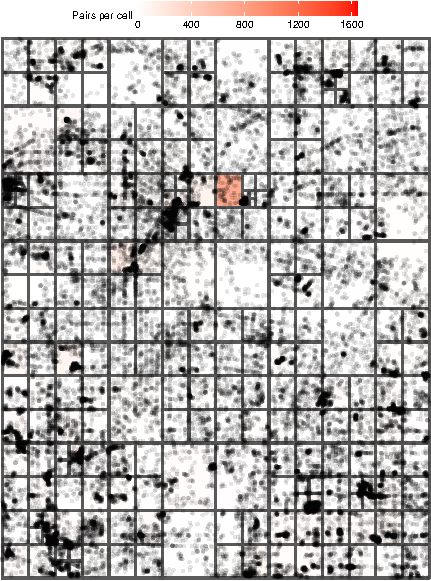
\includegraphics[width=1\linewidth,height=0.8\textheight]{distance_files/figure-latex/p2_318_500_4-1} 

\end{minipage}

\pagebreak

\hypertarget{time-instant-318-capacity1000-leafs127-epsilon4.}{%
\subsection{Time instant : 318 (capacity=1000, leafs=127,
epsilon=4).}\label{time-instant-318-capacity1000-leafs127-epsilon4.}}

\begin{minipage}{0.5\textwidth} 
\centering 
\begin{tabular}{rrrrrrr}
  \hline
 & Min. & 1st Qu. & Median & Mean & 3rd Qu. & Max. \\ 
  \hline
stats & 4.00 & 210.50 & 351.00 & 400.19 & 548.00 & 990.00 \\ 
   \hline
\end{tabular}
\vspace{0.5cm} 


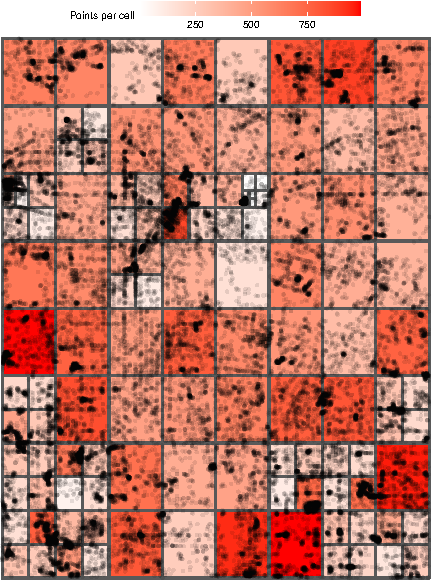
\includegraphics[width=1\linewidth,height=0.8\textheight]{distance_files/figure-latex/p1_318_1000_4-1} 

\end{minipage} 
\begin{minipage}{0.5\textwidth} 
\centering 
\begin{tabular}{rrrrrrr}
  \hline
 & Min. & 1st Qu. & Median & Mean & 3rd Qu. & Max. \\ 
  \hline
stats & 0.00 & 8.00 & 18.00 & 79.78 & 41.50 & 1649.00 \\ 
   \hline
\end{tabular}
\vspace{0.5cm} 


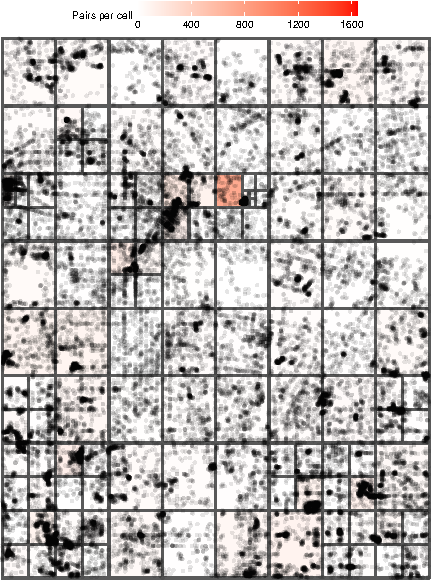
\includegraphics[width=1\linewidth,height=0.8\textheight]{distance_files/figure-latex/p2_318_1000_4-1} 

\end{minipage}

\pagebreak

\hypertarget{time-instant-318-capacity1500-leafs85-epsilon4.}{%
\subsection{Time instant : 318 (capacity=1500, leafs=85,
epsilon=4).}\label{time-instant-318-capacity1500-leafs85-epsilon4.}}

\begin{minipage}{0.5\textwidth} 
\centering 
\begin{tabular}{rrrrrrr}
  \hline
 & Min. & 1st Qu. & Median & Mean & 3rd Qu. & Max. \\ 
  \hline
stats & 4.00 & 317.00 & 538.00 & 595.49 & 816.00 & 1431.00 \\ 
   \hline
\end{tabular}
\vspace{0.5cm} 


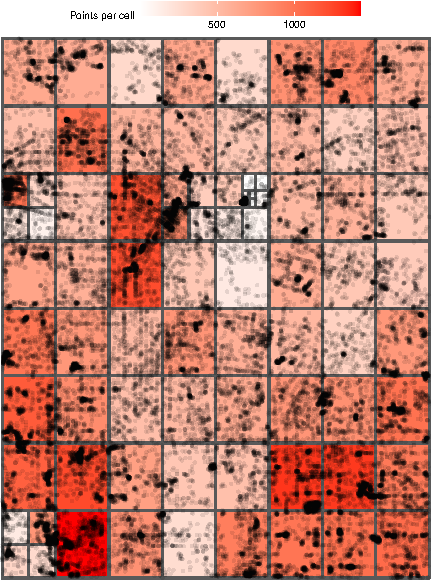
\includegraphics[width=1\linewidth,height=0.8\textheight]{distance_files/figure-latex/p1_318_1500_4-1} 

\end{minipage} 
\begin{minipage}{0.5\textwidth} 
\centering 
\begin{tabular}{rrrrrrr}
  \hline
 & Min. & 1st Qu. & Median & Mean & 3rd Qu. & Max. \\ 
  \hline
stats & 0.00 & 9.00 & 27.00 & 114.28 & 80.00 & 3892.00 \\ 
   \hline
\end{tabular}
\vspace{0.5cm} 


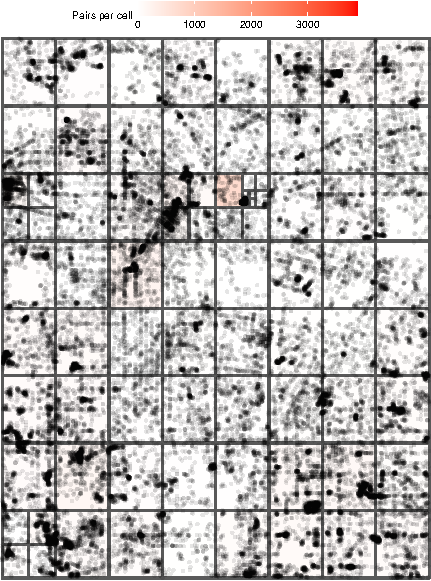
\includegraphics[width=1\linewidth,height=0.8\textheight]{distance_files/figure-latex/p2_318_1500_4-1} 

\end{minipage}

\pagebreak

\end{document}
